\section{Rotation}\label{Sec:Rotation}
To handle rotation in \maestro\ we move to the co-rotating reference frame.  Time
derivatives of a vector in the inertial frame are related to those in the 
co-rotating frame by
\begin{equation}\label{eq:derivative relations}
  \left(\frac{D}{Dt}\right)_\text{i} = 
  \left[\left(\frac{D}{Dt}\right)_\text{rot} + \Omegab\times\ \right],
\end{equation}
where i(rot) refers to the inertial(co-rotating) frame and $\Omegab$ is
the angular velocity vector.  Using (\ref{eq:derivative relations}) and 
assuming $\Omegab$ is constant, we have
\begin{equation}\label{eq:rotational velocity relation}
  \frac{Dv_\text{i}}{Dt} = \frac{Dv_\text{rot}}{Dt} + 
  2\Omegab \times \mathbf{v_\text{rot}} +
  \Omegab\times\left(\Omegab\times r_\text{rot}\right).
\end{equation}
Plugging this into the momentum equation and making use of the continuity 
equation we have a momentum equation in the co-rotating frame:
\begin{equation}\label{eq:momentum equation with rotation}
  \frac{\partial(\rho\mathbf{U})}{\partial t} + 
  \nabla\cdot\left(\mathbf{U}(\rho\mathbf{U}) + p \right) = 
  \underbrace{-2\rho\Omegab\times\mathbf{U}}_{\text{Coriolis}} -
  \underbrace{\rho\Omegab\times\left(\Omegab\times
    \rb\right)}_{\text{Centrifugal}} - 
  \rho \mathbf{g}.
\end{equation}
The Coriolis and Centrifugal terms are force terms that will be added to 
right hand side of the equations in {\tt mk\_vel\_force}.  Note that the 
Centrifugal term can be rewritten as a gradient of a potential and absorbed
into either the pressure or gravitational term to create an effective pressure
or effective gravitational potential.  Furthermore, because it can be written
as a gradient, this term would drop out completely in the projection if we were
doing incompressible flow.\MarginPar{Is this how John stated it?}
In what follows we will include the Centrifugal term explicitly.

\subsection{Using Spherical Geometry}\label{Sec:Using Spherical Geometry}
In spherical geometry implementing rotation is straightforward as we don't have
to worry about special boundary conditions.  We assume a geometry as shown in
Figure \ref{Fig:rotation in spherical} where the primed coordinate system is 
the simulation domain coordinate system, the unprimed system is the primed 
system translated by the vector $\rb_\text{c}$ and is added here for
clarity.  The  $\rb_\text{c}$ vector is given by {\tt center} in the 
{\tt geometry} module.  In spherical, the only runtime parameter of importance
is {\tt rotational\_frequency} in units of Hz.  This specifies the angular 
velocity vector which is assumed to be along the {\bf k} direction:
\[
\Omegab \equiv \Omega \text{\bf k} = 2\pi *
\left(\text{\tt rotational\_frequency}\right)\text{\bf k}.
\]
The direction of $\rb$ is given as the {\tt normal} vector which is 
passed into {\tt mk\_vel\_force}; in particular
\[
\cos\theta \equiv \frac{\rb\cdot\text{\bf k}}{r} = 
\text{\bf normal}\cdot\text{\bf k} = \text{\tt normal}(3).
\]
The magnitude of $\rb$ is calculated based on the current zone's location with
respect to the {\tt center}.
Using this notation we can write the Centrifugal term as
\begin{align*}
\Omegab\times\left(\Omegab\times\rb\right) &=
\left(\Omegab\cdot\rb\right)\Omegab - \left(\Omegab\cdot\Omegab\right)\rb\\
&= \Omega^2 r *\left[\text{\tt normal}(3)\right]\text{\bf k} -
\Omega^2 r *\text{\bf normal} = \left(
\begin{array}{c}
\Omega^2r*\left[\text{\tt normal}(1)\right]\\
\Omega^2r*\left[\text{\tt normal}(2)\right]\\
0 \end{array}\right).
\end{align*}
The Coriolis term is a straightforward cross-product:
\begin{align*}
\Omegab \times \Ub &= \left|
\begin{array}{ccc}
  \text{\bf{i}}&\text{\bf{j}}&\text{\bf{k}}\\
  0 & 0 & \Omega\\
  u & v & w
\end{array}\right|\\
&= \left(
\begin{array}{c}
-\Omega v\\ \Omega u \\ 0
\end{array}
\right).
\end{align*}

%%%%%%%%%%%%%%%%%%%%%%%%%%%%%%%%%
\begin{figure}[tpb]
\hspace{-0.25in}
\centering
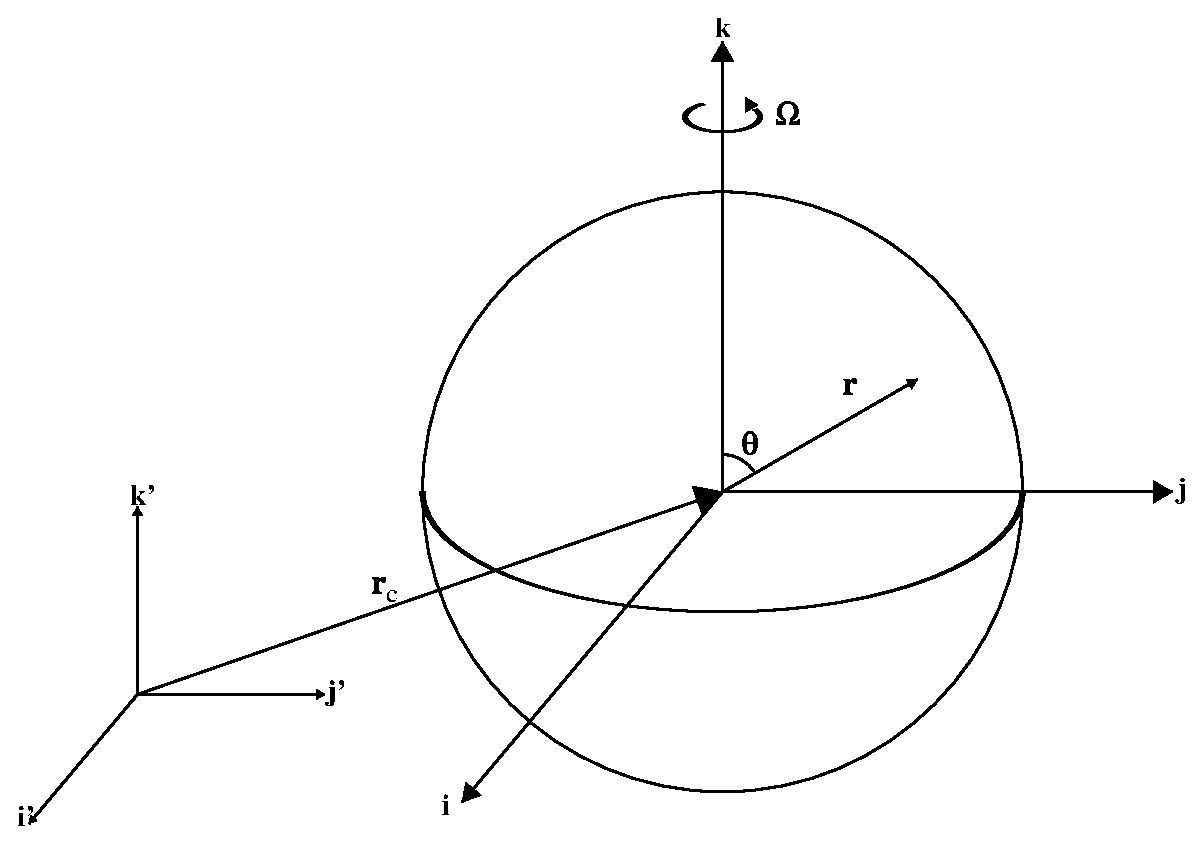
\includegraphics[width=4.5in]{\rotfigpath/rotation_spherical}
\begin{minipage}[h]{2.0in}
\vspace{-4in}
\caption[Rotation geometry]
{Geometry of rotation when {\tt spherical\_in} $=1$.  We assume the 
star to be rotating about the $z$ axis with rotational frequency $\Omega$.}
\end{minipage}
\label{Fig:rotation in spherical}
\end{figure}
%%%%%%%%%%%%%%%%%%%%%%%%%%%%%%%%%

\subsection{Using Plane-Parallel Geometry}\label{Sec:Using Plane-Parallel Geometry}
